\section{Woche 4 - AK OpenSource \headerand OpenSource Forum Erfurt} \label{sec:bericht-wo-4}

% Woche 4 (2023-09-25 bis 2023-09-29)

\lweekdaymarginpar{\weekdayMondayLong}

Montag besprach ich dann mit meinem Chef noch die letzten Unklarheiten.
Einen der Teile der Präsentation konnte ich an meinen Chef abgeben, da ich mich mit diesem einen Thema nicht sonderlich gut auskannte.
Den Rest des Tages nutzte ich lieber Zuhause im Home-Office, um die Präsentation in Ruhe üben und meine Reisetasche für die morgige Reise nach Erfurt packen zu können.

\sweekdaymarginpar{\weekdayTuesdayLong}

Der Dienstag begann früh mit unserer Reise mit dem ICE nach Erfurt, die mein Chef und ich für eine letzte Durchsprache nutzten.
Angekommen in Erfurt ging es direkt in den nahegelegenen Räumlichkeiten der DB Systel, wo es zunächst einleitende Worte und eine Vorstandswahl gab.
Im Anschluss daran war ich mit meiner Präsentation dran, bei der trotz anfänglicher Nervosität alles reibungslos verlief:
Ich brauchte mein Skript kaum und das Feedback war ausschließlich positiv, was mich sehr gefreut hat, denn ich wollte einen Mehrwert in diese Runde bringen.

Abends wurde vom {\bitkom} eine Stadtführung und ein gemeinsames Abendessen mit anderen Teilnehmern des OpenSource Forums organisiert, an welchen wir teilnahmen.
So konnten wir uns auch mit den anderen Teilnehmern austauschen.

\sweekdaymarginpar{\weekdayWednesdayLong}

Das OpenSource Forum der {\bitkom} bot eine entspannte Alternative zum vorherigen Tag, bei dem die Teilnehmer vielfältige Präsentationen verfolgen und sich untereinander auszutauschen konnten.
Besonders spannend waren die Einblicke in die Open-Source-Strategien großer Unternehmen wie SAP, Siemens und Mercedes.
Die Parallelen im Bezug auf die aktuellen Herausforderungen und Lösungsansätze für die Verwaltung von Schwachstellen und Lizenzen von Open-Source-Software in ihren Produkten und Projekten haben mich etwas überrascht und bestätigten die Relevanz unserer Arbeit.

\begin{figure}[htbp] % here, top, bottom, separate page
    \centering
    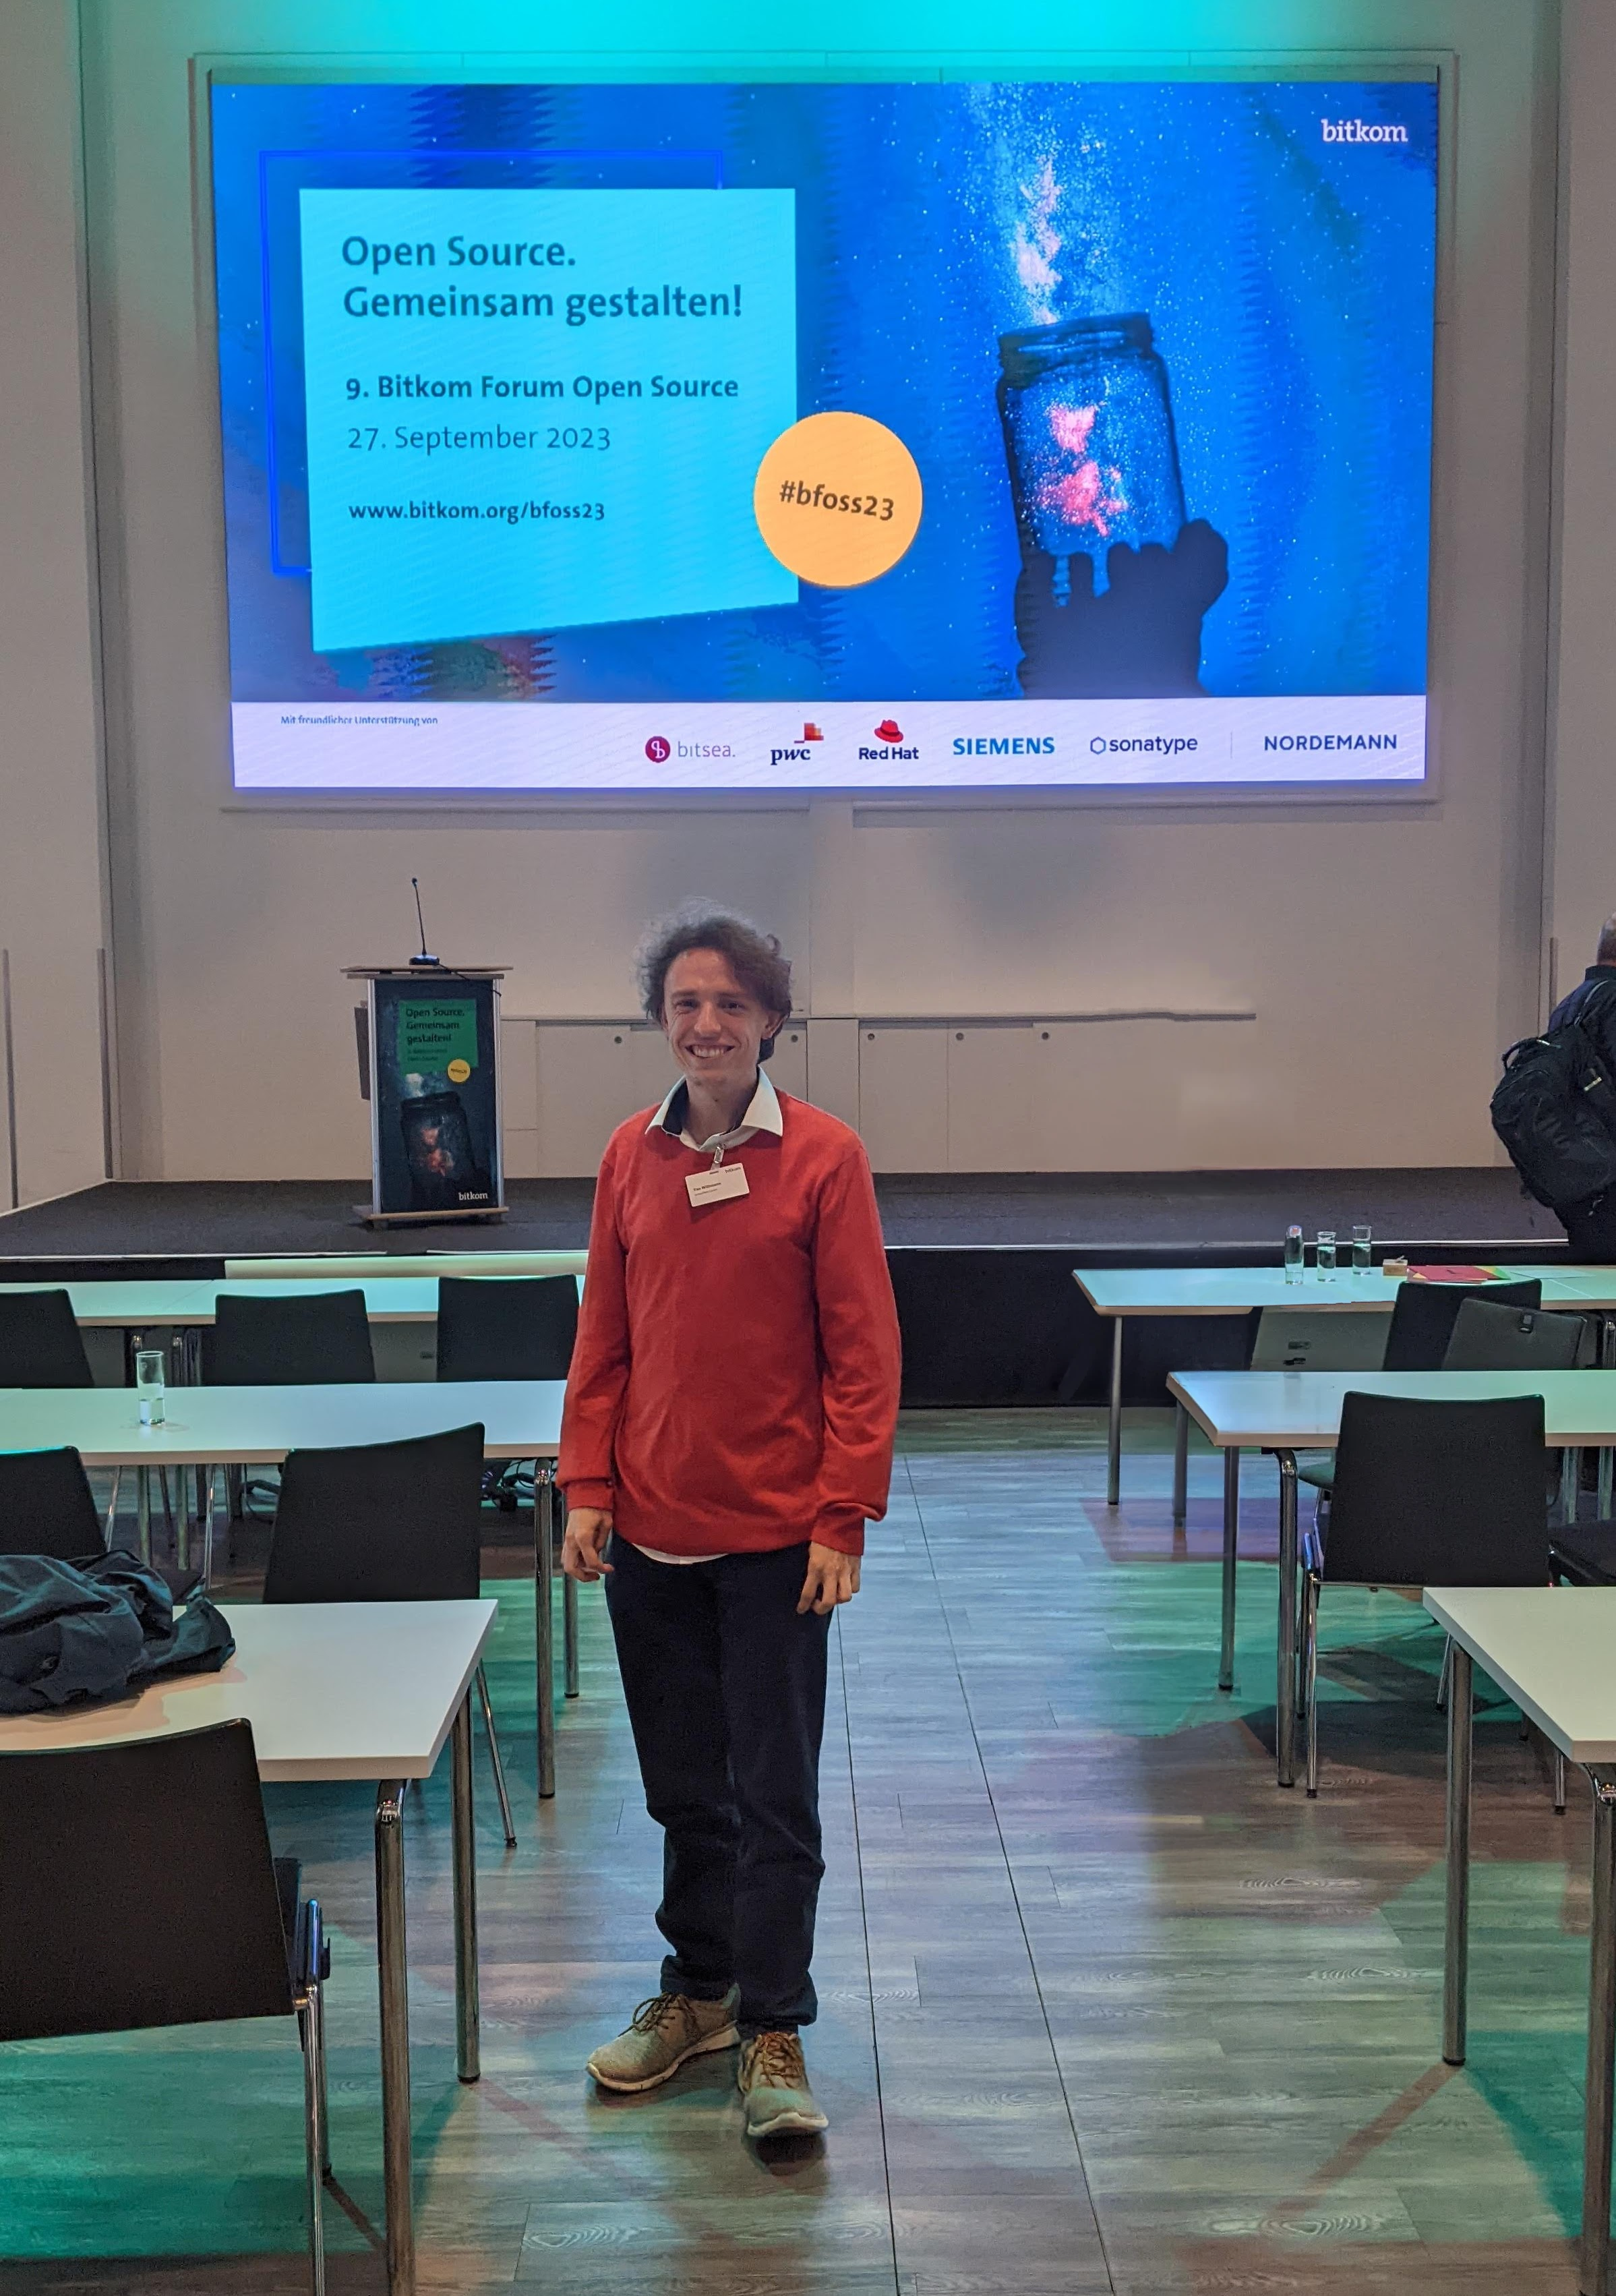
\includegraphics[width=0.5\textwidth, keepaspectratio]{res/img/2023-10-19-yan-ak-os}
    \caption{Auf dem Forum Open Source der Bitkom 2023}
    \label{fig:foss23-yan}
\end{figure}

Ein großer Programmpunkt war auch der {\bitkom} OpenSource Monitor\footnote{\url{https://www.bitkom.org/opensourcemonitor2023}}, der durch {\metaeffekt} gesponsert wird, wie in Abbildung \ref{fig:foss23-sponsor-metaeffekt} zu sehen ist.
Damit durfte die {\metaeffekt} einen Beitrag über den Cyber Resilience Act\footnote{\url{https://digital-strategy.ec.europa.eu/en/policies/cyber-resilience-act}} verfassen, der in diesem abgedruckt wurde.
Auch einige unserer direkten Kunden waren vertreten, die ich noch nie in Person getroffen hatte, außerdem konnte ich mit Studenten und Angestellten verschiedener Unternehmen sprechen.

\begin{figure}[htbp] % here, top, bottom, separate page
    \centering
    \includegraphics[width=0.8\textwidth, keepaspectratio]{res/img/2023-10-19-ak-os-metaeffekt-sponsor}
    \caption{Die {\metaeffekt} ist links als Sponsor zum OpenSource Monitor aufgeführt}
    \label{fig:foss23-sponsor-metaeffekt}
\end{figure}

\sweekdaymarginpar{\weekdayThursdayShort, \weekdayFridayShort}

Die Rückreise am Donnerstag verlief ohne Zwischenfälle, sodass der Freitag wieder der gewöhnliche Arbeitsalltag war.
Eine neue Kundenanforderung erforderte schon wieder direkte Aufmerksamkeit:
Einer unserer Download-Prozesse scheitert in ihrer Konfiguration, da der verwendete git-Befehl die konfigurierte Proxy-Informationen bislang scheinbar ignoriert.
Um das zu lösen, kann Git sowohl über einen Konfigurationsparameter im Befehlsaufruf, als auch über Umgebungsvariablen der Session konfiguriert werden.
Ich habe mich für die zweite Variante entschieden.

Ein persönliches Highlight war diesen Freitag allerdings, dass mein Bruder ab nächster Woche auch Teil des {\metaeffekt} Teams sein wird.
